\documentclass[a4paper]{jpconf}
\usepackage{graphicx}

\newcommand{\athenamp}{\texttt{AthenaMP}}
\newcommand{\athenamt}{\texttt{AthenaMT}}
\newcommand{\gaudi}{\textsc{Gaudi}}
\newcommand{\athena}{\textsc{Athena}}
\newcommand{\python}{\texttt{python}}
\newcommand{\cython}{\texttt{cython}}
\newcommand{\golang}{\texttt{Go}}
\newcommand{\henp}{\texttt{HENP}}
\newcommand{\linux}{\texttt{GNU/Linux }}
\newcommand{\goroutine}{\texttt{goroutine}}
\newcommand{\goroutines}{\texttt{goroutines}}

% for code colouring
\usepackage{pgf,pgfarrows,pgfnodes,pgfautomata,pgfheaps,pgfshade}
\usepackage{amsmath,amssymb}
\usepackage[latin1]{inputenc}
\usepackage{colortbl}
\usepackage[procnames]{listings}
%\include{pythonlisting}
%\include{cpplisting}
%%%%%%%%%%%%%%%%%%%%%

\begin{document}
\title{ng: What next-generation languages can teach us about
  \henp\ frameworks in the manycore era}

\author{S\'ebastien Binet}

\address{Laboratoire de l'Acc\'el\'erateur Lin\'eaire, Universit\'e
  Paris-Sud XI, 91898, Orsay, FR}

\ead{binet@cern.ch}

\begin{abstract}

Current High Energy and Nuclear Physics (\henp ) frameworks were
written before multicore systems became widely deployed.
A 'single-thread' execution model naturally emerged from that
environment, however, this no longer fits into the processing model on
the dawn of the manycore era.
Although previous work focused on minimizing the changes to be applied
to the LHC frameworks (because of the data taking phase) while still
trying to reap the benefits of the parallel-enhanced CPU
architectures, this paper explores what new languages could bring to
the design of the next-generation frameworks.

Parallel programming is still in an intensive phase of R\&D and no
silver bullet exists despite the 30+ years of literature on the
subject.
Yet, several parallel programming styles have emerged: actors, message
passing, communicating sequential processes, task-based programming,
data flow programming, \ldots to name a few.

We present the work of the prototyping of a next-generation framework
in new and expressive languages (\python\ and \golang\ ) to
investigate how code clarity and robustness are affected and what are
the downsides of using languages younger than
\textsc{Fortran}/\texttt{C}/\texttt{C++}.
\end{abstract}

\section{Introduction}

The \emph{``Free Lunch''} is over: Moore's law~\cite{ref-moore} can
not be as easily leveraged as in the past, computer scientists and
software writers have now to be familiar with Amdahl's
law~\cite{ref-amdahl}.
Indeed, computers are no longer getting faster: instead, they are
growing more and more {\tt CPU}s, each of which is no faster than the
previous generation. 

This increase in the number of cores evidently calls for more parallelism in \henp\ software.
Fortunately, typical \henp\ applications (event reconstruction,
event selection,...) are usually \emph{embarrassingly parallel}, at
least at the coarse-grained level: one ``just'' needs to call in parallel
the portion of code which massages the events retrieved from the
detector (the event loop) while still executing sequentially all the
code processing each event.

However, the strategy devised and implemented in
\athenamp~\cite{ref-athenamp} where the {\tt fork} system call and the
\emph{Copy-On-Write (COW)} mechanism were leveraged in order to save memory
footprint and use multiple cores will probably not scale up to manycore
systems as \emph{COW}'s efficiency is bounded as well as the amount of
\emph{RAM} available on a given machine.
Indeed, the amount of physical memory associated to a core will not
scale with the increasing number of cores.
A 'one-event/one-core/one-process' strategy, even if \linux has
this codepath optimized, will bring the machine on its knees when
thousands of cores will be available, especially if each of these
processes perform a non-negligible amount of (possibly chaotic) I/O.

Therefore, it seems more efficient to have at least the
event-level~\footnote{\emph{i.e.:} as opposed to \emph{e.g.} a
  conditions-level data} data parallel processing being performed in
the same address space.
In a {\tt C++} world, this means multithreading and raises all the issues
already noted during the development of \athenamt~\cite{ref-athenamp}:
\begin{itemize}
\item it is hard to get a multithreaded application right,
\item hard to keep it right,
\item hard to keep it efficient and optimized across releases.
\end{itemize}

Even if the next version of {\tt C++}~\cite{ref-cxx} will improve the
situation with {\tt lambda}s, {\tt std::future} and {\tt std::thread},
at least on the standardization and portability fronts, this will be
achieved at the cost of complicating further the language.
At this point, it would seem reasonable to ask if using a new language
more capable at leveraging multithreaded environments would be a more
reasonable alternative.

This paper explores such a path.
We first recall the basic architecture of the \gaudi~\cite{ref-gaudi}
framework to identify the main components which would need
modifications in a multithreaded environment.
Then, after motivating why we chose \golang, we will introduce some of its
most relevant features with regard to concurrency and how these have
been translated into a new \golang-based framework, {\tt ng-go-gaudi}.
Finally, after having presented scalability results, we will draw
some conclusions and propose ideas on future work and possible
improvements to {\tt ng-go-gaudi}.

\section{{\sc Athena/Gaudi} refresher}
\gaudi~\cite{ref-gaudi} is an object-oriented {\tt C++}-based software
framework built around the \emph{Component Object Model
  (COM)}~\cite{ref-com}.
\emph{Data} objects (event data, detector data or statistical data)
are recorded into and retrieved from a component: the \emph{data
  store}.
\emph{Algorithm} objects are the components which manipulate this data or
create new and more refined data quantities by interacting with the
\emph{data store}.
The creation of these algorithms and proper state transitions are
ensured and orchestrated by a central service, the {\tt
  ApplicationManager}, while the in-order scheduling of the algorithms
is managed by the {\tt EventLoopManager}, as schematized in figure~\ref{gaudi-com}.

\begin{figure}[h]
\begin{center}
  \begin{minipage}{17pc}
    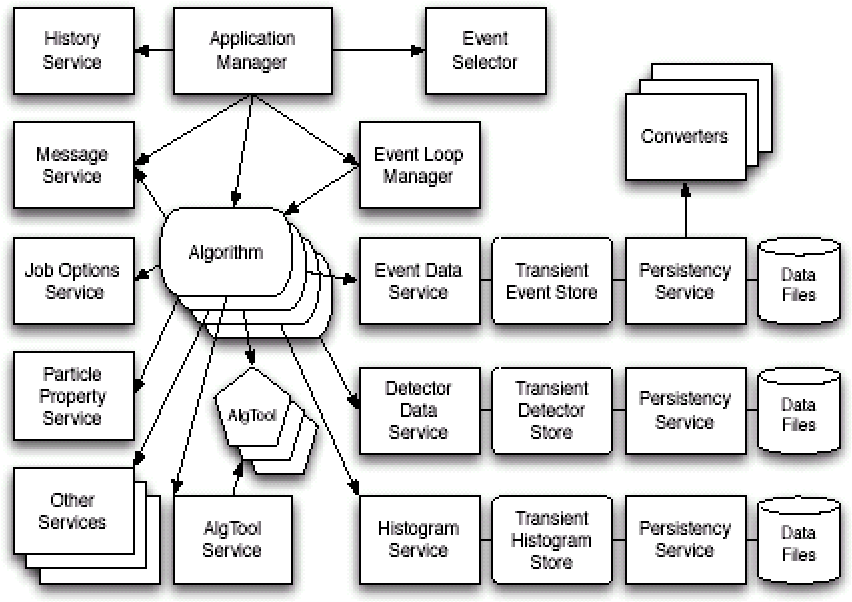
\includegraphics[width=14pc]{figs/athena-component-model.pdf}
    \caption{\label{gaudi-com}Overview of the \gaudi\ framework. At the
    center are the multiple algorithms, interacting with many core
    services ({\tt Event Data Service, JobOptionsSvc},\ldots) and
    being scheduled by the {\tt EventLoopManager} which is itself
    steered by the {\tt ApplicationManager}.}
  \end{minipage}\hspace{2pc}%
  \begin{minipage}{15pc}
\begin{lstlisting}[language=c++,
    basicstyle=\tiny,
    frame=trbl,
    numbers=left,
    showstringspaces=false,
    stringstyle=\ttfamily]
class IAlgorithm : public IInterface { 
  public:
   virtual StatusCode initialize() = 0;
   virtual StatusCode execute() = 0;
   virtual StatusCode finalize() = 0;
};
\end{lstlisting}
\caption{\label{gaudi-alg}{\tt C++ Algorithm} interface.}
%  Concrete classes will have to implement the {\tt execute()} method which is
%  called by the framework for each event to process.}
    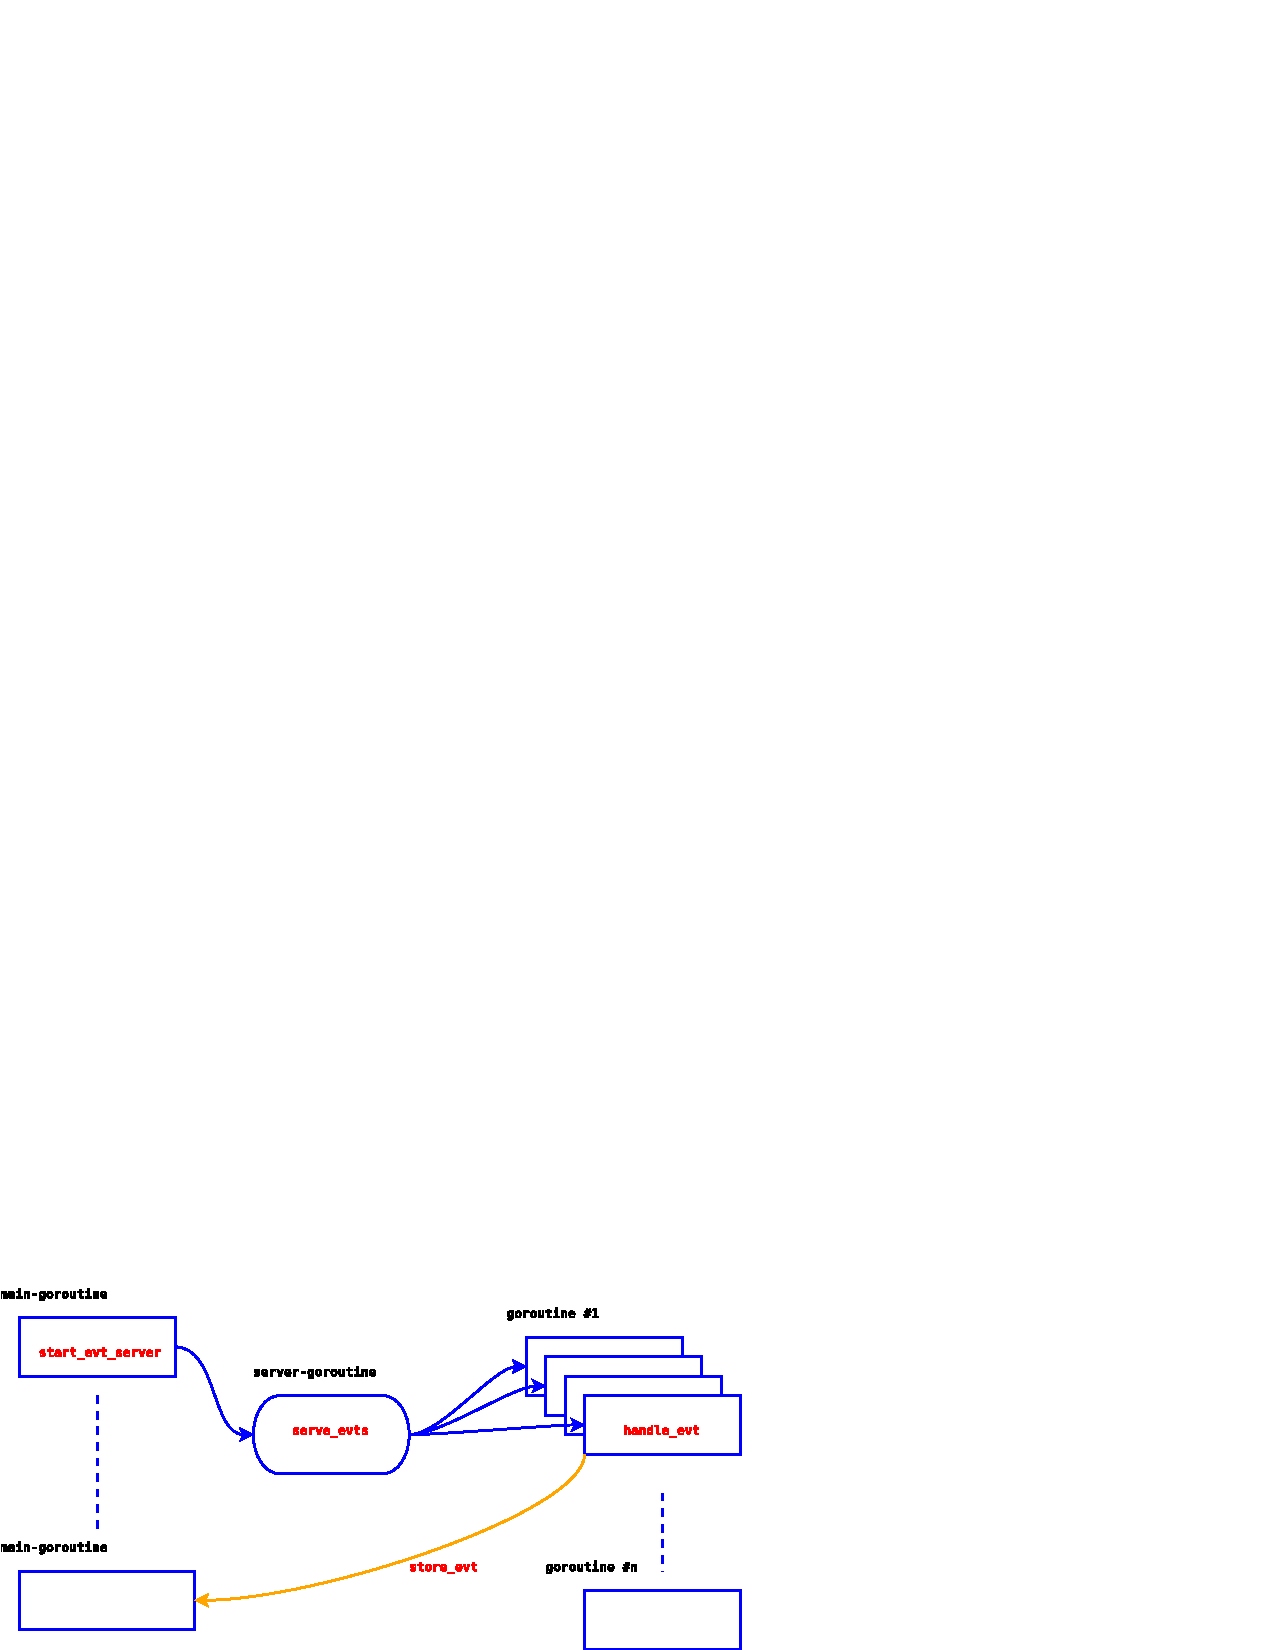
\includegraphics[width=14pc]{figs/evtproc-diagram.pdf}
    \caption{\label{fig-mp-evt-loop}Overview of the parallelized event
      processor.}
  \end{minipage} 
\end{center}
\end{figure}

As can be seen in figure~\ref{gaudi-com}, the workhorse component is
the {\tt Algorithm} one whose (simplified) interface is reported in
figure~\ref{gaudi-alg}.
The {\tt execute()} method is called for each event and usually
involves retrieving data from the event store as well as recording new
more refined data in that event store.
Previous work~\cite{ref-athenamp} focused on maintaining that
interface, while modifying the framework behind the scene to leverage
the {\tt fork()} and \emph{COW} mechanisms to transparently
parallelize the \gaudi\ application at the event level.

Keeping these key elements in mind, we now investigate what a
\gaudi-like framework would probably look like if it were written in a
new more parallel- or concurrent-friendly language.

\section{New languages}
Since \henp\ and {\tt C++} met to produce (among other projects)
\gaudi\ and {\tt ROOT}~\cite{ref-root}, the language landscape greatly
changed.
Many new languages appeared or became \emph{``mainstream''} and, while
closely following the trend was not achieved, some adaptations were performed.
For example, most of the \gaudi\ configuration and steering code is
nowadays written in \python\ and most, if not all, {\tt C++} components
(from {\tt ROOT} and \gaudi) are also available from \python.
But \python\ (or more precisely {\tt CPython}) has well-known
scalability issues in a multithreaded environment because of its
\emph{Global Interpreter Lock (GIL)} which serializes access to
\python\ objects~\footnote{Other \python\ implementations
  (\texttt{JPython}, \texttt{IronPython},\ldots) do not
  present this limitation.}.
Moreover, even if this issue can be worked around by writing {\tt C}
extension modules, having an event loop in an interpreted language
is not the best bet CPU-speed wise.

Other languages such as \textsc{Haskell}~\cite{ref-haskell} have been
considered for this study.
Indeed, functional languages are a great substrate for automated code
parallelization~\cite{ref-auto-parallel-fp} thanks to their \emph{``no
  side effects''}~\footnote{this is true for the so-called \emph{pure}
functional languages.} property, sidestepping race conditions.
However, functional programming languages are probably not yet fitting
into the average physicist software toolbox, with problems on their own
(such as space leaks stemming from the laziness of \textsc{Haskell})
lacking proper tools to debug, and were thus discarded from this study.
\texttt{Vala}~\cite{ref-vala} was considered because of its support
for interfaces, which match very well the \gaudi\ COM architecture, as
well as for its ability to asynchronously start tasks and co-routines.
However, the lack of documentation and the fact that ``only''
\textsc{Gnome} is using this language, disqualified it for this
study.

We were hence left with \golang.

\subsection{Elements of \golang}
\golang~\cite{ref-golang} is a new open source language from Google,
first released in November 2009.
It is a compiled language with a garbage collector and builtin support
for reflection, first-class functions, closures and object-oriented
programming.
%% The obligatory \emph{``hello world''} program can be found in
%% figure~\ref{fig-hello-world}.

%% \begin{figure}[h]
%% \begin{center}
%% \begin{lstlisting}[language=Go,
%%     basicstyle=\small,
%%     frame=trbl,
%%     numbers=left,
%%     showstringspaces=false,
%%     stringstyle=\ttfamily]
%% package main
%% import "fmt"
%% func main() {
%%     fmt.Println("Hello, world")
%% }
%% \end{lstlisting}
%% \end{center}
%% \caption{\label{fig-hello-world}The obligatory \emph{``hello world''}
%%   program, in \golang.}
%% \end{figure}

\golang\ is lauded to bring the best of both dynamic and static worlds:
\begin{itemize}
\item the feel of a dynamic language, thanks to its limited verbosity,
  its type inference system and its fast compile-edit-run cycle,
\item the safety of a static type system,
\item the speed of a machine compiled language.~\footnote{the aim of
  the \golang\ authors is to eventually bring the performances of a
  \golang\ binary within $10\%$ of \texttt{C}.}
\end{itemize}

Moreover, \golang\ support for interfaces which resembles the
\emph{duck-typing} motto of \python\ fits nicely into the \gaudi\
framework.
Finally and more importantly, \golang\ has language support for
concurrency, modelled after the \emph{Communicating Sequential Processes
  (CSP)}~\cite{ref-csp} model: prefixing a method or function call
with the keyword \texttt{go} will spawn off a \goroutine: the
function will be executed concurrently to other codepaths.
\goroutines\ are multiplexed onto multiple OS threads so
blocked \goroutines\ because of a non-finished I/O operation
will not halt the execution of the others.
Furthermore, \goroutines\ are lightweight thanks to their
variable stack size, starting small and growing as needed.

In \golang, the typesafe mechanism to exchange data between
\goroutines, is called \emph{channel}.
Sending or receiving data on a channel is atomic and can thus be used
as a synchronization mechanism.
It should be noted that as of 2010, \golang\ is lacking a few features
which would probably make the current implementation of
\texttt{ng-go-gaudi} a bit easier, such as dynamic libraries and
dynamic code loading.
Another set of missing features more important for efficient
scientific code is the lack of generics~\footnote{also called
  templates in \texttt{C++}.} and the lack of operators overloading.

\section{\texttt{ng-go-gaudi} implementation}
\texttt{ng-go-gaudi} is a \golang\ implementation of a minimal
framework modeled after \gaudi.

The current implementation can be found in a \verb'Mercurial'
repository~\cite{ref-ng-go} and holds:

\begin{itemize}
  \item an application manager, an event processor, and a data store
    service, 
  \item base classes for algorithms with support for messaging and
    configuration \emph{via} properties,
  \item a simple \texttt{JSON} output stream and a simple
    \golang\ bytestream (\texttt{gob}) output stream, 
  \item and few simple test algorithms (\texttt{adder},
    \texttt{counter}, \ldots).
\end{itemize}
 
\subsection{Parallelizing the event loop}
Leveraging the \emph{embarassingly parallel} nature of the typical
\henp\ application, the event processor was parallelized, following
the ideas of \athenamp\ and \athenamt.
The overall architecture of this parallelization is schematized in
figure~\ref{fig-mp-evt-loop} and the code to achieve it is reproduced
in figure~\ref{fig-evt-proc-code}.
Lines $23$ to $33$ setup a server \goroutine\ which will take a
buffered~\footnote{The input queue is buffered to limit the number of
  in-flight events.This can of course be configured at the command
  line level.} input queue of events to process and (eventually)
asynchronously call an event handling function to process the events. 
These processed events will then be removed from the input queue and
will appear on the output one.
Following a typical concurrent \golang\ pattern, a third
\emph{channel}, the \texttt{quit} one, is also created to notify
clients when the event source is done, allowing to cleanly terminate the event processing.
be cleanly terminated.

\begin{figure}[h]
\begin{center}
  \begin{minipage}{18pc}
\begin{lstlisting}[language=Go,
    basicstyle=\tiny,
    frame=trbl,
    numbers=left,
    showstringspaces=false,
    stringstyle=\ttfamily]
func (self *evtproc) 
mp_NextEvent(evtmax int) kernel.Error {
  handle := func(evt *evtstate, 
                 out_queue chan <- *evtstate) {
    evt.sc = self.ExecuteEvent(evt)
    out_queue <- evt
  }

  serve_evts := func(
    in_evt_queue <- chan *evtstate, 
    out_evt_queue chan <- *evtstate, 
    quit <- chan bool) {
    for {
      select {
        case ievt := <-in_evt_queue:
          go handle(ievt, out_evt_queue)
        case <-quit:
          return
      }
    }
  }

  start_evt_server := func(nworkers int) 
    (in_evt_queue,
     out_evt_queue chan *evtstate,
     quit chan bool) {
    in_evt_queue = make(chan *evtstate, nworkers)
    out_evt_queue = make(chan *evtstate)
    quit = make(chan bool)
    go serve_evts(in_evt_queue, out_evt_queue, 
                  quit)
    return in_evt_queue, out_evt_queue, quit
  }

  in_evt_queue, out_evt_queue, quit \
    := start_evt_server(self.nworkers)
  for i:=0; i<evtmax; i++ {
    in_evt_queue <- new_evtstate(i)
  }
  // ...
  return kernel.StatusCode(0)
}
\end{lstlisting}
    \caption{\label{fig-evt-proc-code}\golang\ code realizing the
      parallelization of the event loop.}
\begin{lstlisting}[language=Go,
    basicstyle=\tiny,
    frame=trbl,
    numbers=left,
    showstringspaces=false,
    stringstyle=\ttfamily]
package kernel

/// handle to a concurrent output stream
type IOutputStream interface {
  /// write (and possibly commit) 
  /// data to the stream
  Write(data interface{}) Error
  /// closes and flushes the output stream
  Close() Error
}

/// interface to a concurrent output 
/// stream server
type IOutputStreamSvc interface {
  /// returns a new output stream
  NewOutputStream(stream_name string)
    IOutputStream
}
\end{lstlisting}
    \caption{\label{fig-iout-go}\golang\ interfaces for \gaudi-\texttt{I/O}.}
  \end{minipage}\hspace{3pc}%
  \begin{minipage}{15pc}
\begin{lstlisting}[language=Go,
    basicstyle=\tiny,
    frame=trbl,
    numbers=left,
    showstringspaces=false,
    stringstyle=\ttfamily]
package kernel

type IAlgorithm interface {
  Initialize() Error
  Execute(ctx IEvtCtx) Error
  Finalize() Error
}
\end{lstlisting}
    \caption{\label{fig-ialg-go}Extended \texttt{IAlgorithm} interface.}
\begin{lstlisting}[language=Go,
    basicstyle=\tiny,
    frame=trbl,
    numbers=left,
    showstringspaces=false,
    stringstyle=\ttfamily]
package testalg

import "gaudi/kernel"

type myalg struct {
  kernel.Algorithm
}

func (self *myalg)
Execute(ctx kernel.IEvtCtx) kernel.Error {
  store := self.EvtStore(ctx)
  store.Put("foo", 42)
  return kernel.StatusCode(0)
}
\end{lstlisting}
    \caption{\label{fig-alg-test-go}Example of accessing a particular
      data store in client code.}
\begin{lstlisting}[language=Go,
    basicstyle=\tiny,
    frame=trbl,
    numbers=left,
    showstringspaces=false,
    stringstyle=\ttfamily]
package outstream
import "json"
/// output stream using JSON as a format
type json_outstream_handle struct {
  svc kernel.IService
  w *os.File
  enc *json.Encoder
  data chan interface{}
  errs chan os.Error
  quit chan bool
}

func (self *json_outstream_handle) 
Write(data interface{}) kernel.Error {
  self.data <- data
  select {
    case err := <-self.errs:
      return kernel.StatusCodeWithErr(1, err)
    default:
      return kernel.StatusCode(0)
  }
  return kernel.StatusCode(0)
}
\end{lstlisting}
    \caption{\label{fig-json-out-go}\texttt{JSON} concrete backend.}
  \end{minipage} 

\end{center}
\end{figure}

As shown in figure~\ref{fig-mp-evt-loop}, each event is processed by a
dedicated \goroutine, so the event processing is concurrent.
This means each \goroutine\ needs its own data store and thus each
algorithm needs to know which data store it should interact with.
To fulfill that requirement, the \gaudi\ algorithm interface had to be
extended to encode the data provenance and make the event context
explicit, as shown in figures~\ref{fig-ialg-go} and~\ref{fig-alg-test-go}.

\subsection{Parallel \texttt{I/O}}
\texttt{JSON} and \texttt{gob} output streams have been implemented to
study the feasability of a parallel \texttt{I/O} persistency system.
In each case, the data is transfered from the data store to the
concrete output stream via \emph{channel}s, that data is then owned by
\emph{the} \goroutine\ commiting it to disk.

The \texttt{JSON} service implementation of the
\texttt{NewOutputStream} method of figure~\ref{fig-iout-go} follows
the typical \golang\ pattern already described for the parallel event
loop where three channels are created (input, errors and quit) and a
\goroutine\ which polls on each of these channels.
The \texttt{JSON} output handle is then handed these three channels to
pump data in, as shown in figure~\ref{fig-json-out-go}.

\subsection{Job configuration and results}
As mentioned previously, current (2010) \golang\ does not support
dynamic code loading~\footnote{This limitation should be lifted in a
future \golang\ version.}.
This can be worked around by leveraging the fast compilation of
\golang\ code.
Indeed, \texttt{ng-go-gaudi} job configuration is performed by running
a \python\ script which will generate \golang\ code compiled down to
an executable holding the concrete list of all components to be used
at runtime~\footnote{In \texttt{C++} \gaudi, this is done via
  \texttt{dlopen} and a plugin manager.}.

An excerpt of such a job configuration, scheduling $1000$ algorithms
(incrementing integers and displaying them) multiplexed on $5000$
\goroutines, can be seen in figure~\ref{fig-go-jobo} which, by varying
the number of cores being used at runtime leads to the performance
plot in figure~\ref{fig-go-perfs}. 
The scalability problem which can be observed has been attributed
after inspection of the \goroutines\ profiles to mutex bottlenecks
mainly at the messaging layer: each component can print messages on
screen at various verbosity levels, but as the standard output is
shared between all these components, a contention appears on this
resource.

\begin{figure}[h]
\begin{center}
  \begin{minipage}{20pc}
\begin{lstlisting}[language=python,
    basicstyle=\tiny,
    frame=trbl,
    numbers=left,
    showstringspaces=false,
    stringstyle=\ttfamily]
app.props.EvtMax = 10000
app.props.OutputLevel = 1

app.svcs += Svc("gaudi/kernel/evtproc:evtproc",
                "evt-proc",
                OutputLevel=Lvl.INFO,
                NbrWorkers=5000)

app.svcs += Svc("gaudi/kernel/datastore:datastoresvc", 
                "evt-store")
app.svcs += Svc("gaudi/kernel/datastore:datastoresvc", 
                "det-store")

for i in xrange(500):
    app.algs += Alg("gaudi/tests/pkg2:alg_adder",
                    "addr--%04i" % i,
                    SimpleCounter="my_counter")
    app.algs += Alg("gaudi/tests/pkg2:alg_dumper",
                    "dump--%04i" % i,
                    SimpleCounter="my_counter",
                    ExpectedValue=i+1)
\end{lstlisting}
    \caption{\label{fig-go-jobo}\python\ code used to configure an
      \texttt{ng-go-gaudi} job.}
  \end{minipage}\hspace{2pc}%
  \begin{minipage}{15pc}
    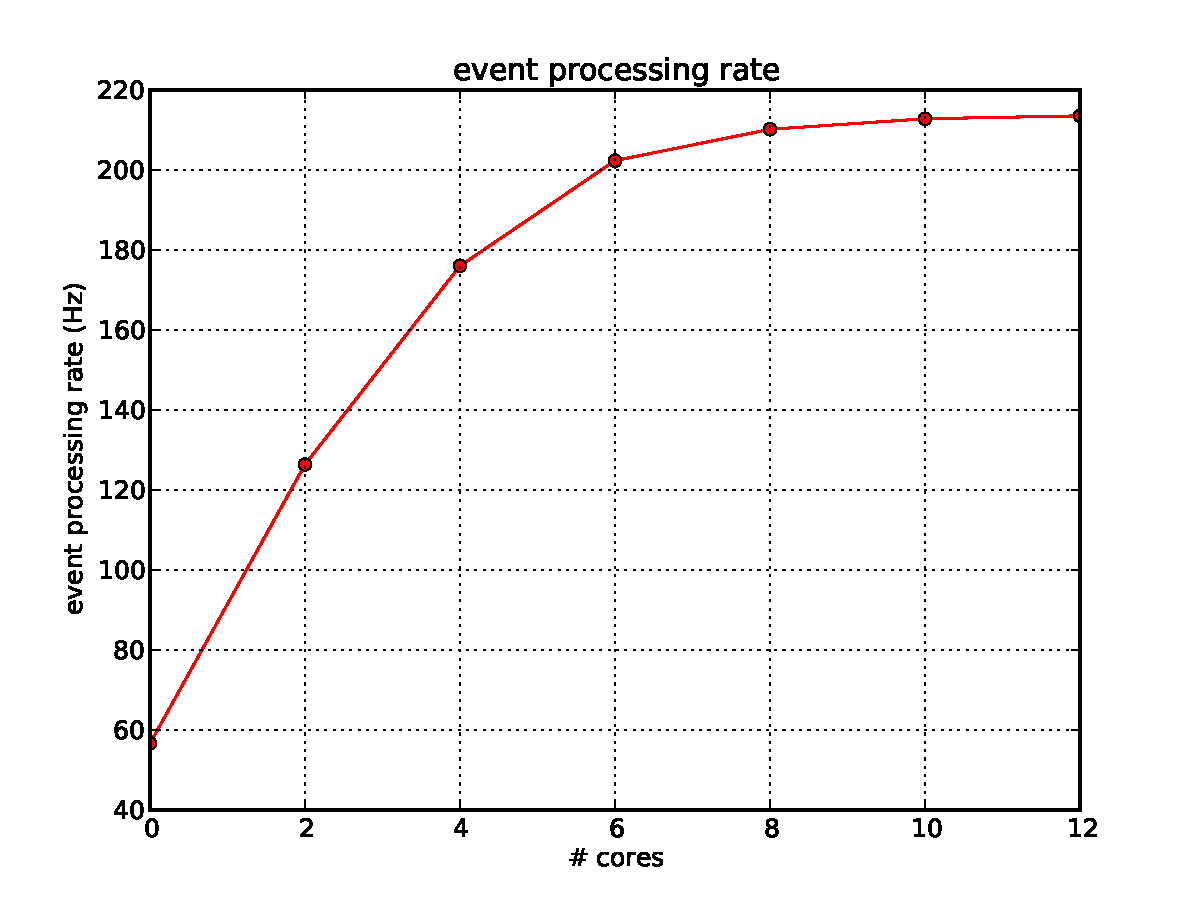
\includegraphics[width=14pc]{figs/perfs.pdf}
    \caption{\label{fig-go-perfs}Event processing rate of an
      \texttt{ng-go-gaudi} application when varying the number of used
      cores.}
  \end{minipage} 
\end{center}
\end{figure}


\section{Conclusions}
We presented a prototype of a \gaudi-like framework written in
\golang\ to investigate what next generation frameworks could look
like when leveraging new languages better tailored at exploiting
concurrency and parallelism.
A concurrent event loop manager and concurrent output streams were
implemented for this study.
Even if some performance problems were uncovered - which could easily be 
addressed by redesigning the \texttt{gaudi/msgstream} to reduce
contention on \texttt{stdout} or by reducing the garbage collector
pressure through a tighter integration with the event loop model of
\gaudi\ - the implementation of concurrent patterns and the ability to
compose them was greatly eased by \golang\ primitives and builtin
support.
We propose to further continue the prototyping of \texttt{ng-go-gaudi}
and address its shortcomings.
Future work will also investigate the feasibility to develop sub-event
concurrency \emph{e.g.} by instrumenting the \texttt{datastore}
accesses to infer a dataflow to allow the parallel execution of algorithms,
and explore ways to improve the memory locality of our big software
framework applications - an obvious way would be to break the single
application into a flock of smaller more specialized ones.

\section*{References}
\begin{thebibliography}{9}
\bibitem{ref-moore} Moore E, "Cramming more components onto integrated circuits'', Electronics Magazine, 1965
\bibitem{ref-amdahl} Amdahl G, "Validity of the Single Processor Approach to Achieving Large-Scale Computing Capabilities", AFIPS Conference Proceedings, (30), pp. 483-485, 1967
\bibitem{ref-gaudi} Mato P 1998 \gaudi-architecture design document Tech. Rep. LHCb-98-064 Geneva
\bibitem{ref-python} The \python\ programming language, \verb'http://python.org'
%\bibitem{ref-cython} \cython, \verb'http://cython.org'
\bibitem{ref-golang} The \golang\ programming language, \verb'http://golang.org/'

\bibitem{ref-athenamp} Binet S, et al. "Harnessing multicores: strategies and
  implementations in \textsc{Atlas}", CHEP, 2009

\bibitem{ref-com} COM, \verb'http://en.wikipedia.org/wiki/Component_Object_Model'

\bibitem{ref-cxx} The \texttt{C++} programming language,
  \verb'http://www.open-std.org/jtc1/sc22/wg21/docs/papers/2010/n3092.pdf'

\bibitem{ref-root} The \texttt{ROOT} framework,
  \verb"http://root.cern.ch"

\bibitem{ref-haskell} The \texttt{Haskell} Programming Language,
  \verb'http://www.haskell.org'

\bibitem{ref-auto-parallel-fp} Harris T, Singh S, "Feedback
  Directed Implicit Parallelism", ICFP, 2007

\bibitem{ref-vala} \texttt{Vala}, \verb'http://live.gnome.org/Vala'
%\bibitem{ref-genie} \texttt{Genie}, \verb'http://live.gnome.org/Genie'

\bibitem{ref-csp} CSP,
  \verb'http://en.wikipedia.org/wiki/Communicating_sequential_processes'

\bibitem{ref-ng-go} \texttt{ng-go-gaudi} \verb'mercurial' repository,
  \verb'http://bitbucket.org/binet/ng-go-gaudi'

\end{thebibliography}

\end{document}


